\section{Resultados}

En este capítulo se exponen los resultados obtenidos tras entrenar las arquitecturas con las modificaciones planteadas. Para poder llevar a cabo un estudio lo más completo posible, se han tomado una serie de valores candidatos para cada modificación (TODO contarles) y se ha llevado a cabo el producto cartesiano de dichos conjuntos, obteniendo así $3 \times 2 \times 3 \times 2 = 36$ modelos distintos.

\todo[inline]{Meter comparación de los tiempos de inferencia con autocast y sin autocast -> Llevar la gráfica al apartado teórico?}

\subsection{Resultados cuantitativos}

\subsubsection{Reducción de tamaño de la entrada}

Dado que el entrenamientos de los modelos - por limitaciones materiales y temporales - se ha llevado a cabo con la entrada del modelo reducida, no es posible realizar una comparación exhaustiva de los resultados obtenidos para cada una de las modificaciones de la arquitectura respecto del modelo correspondiente entrenado con las imágenes en su tamaño original. 

\todo[inline]{Hacer una prueba si cabe en la GPU entrenando solo un modelo}

\begin{wrapfigure}{r}{0.5\textwidth}
\vspace{-10pt}
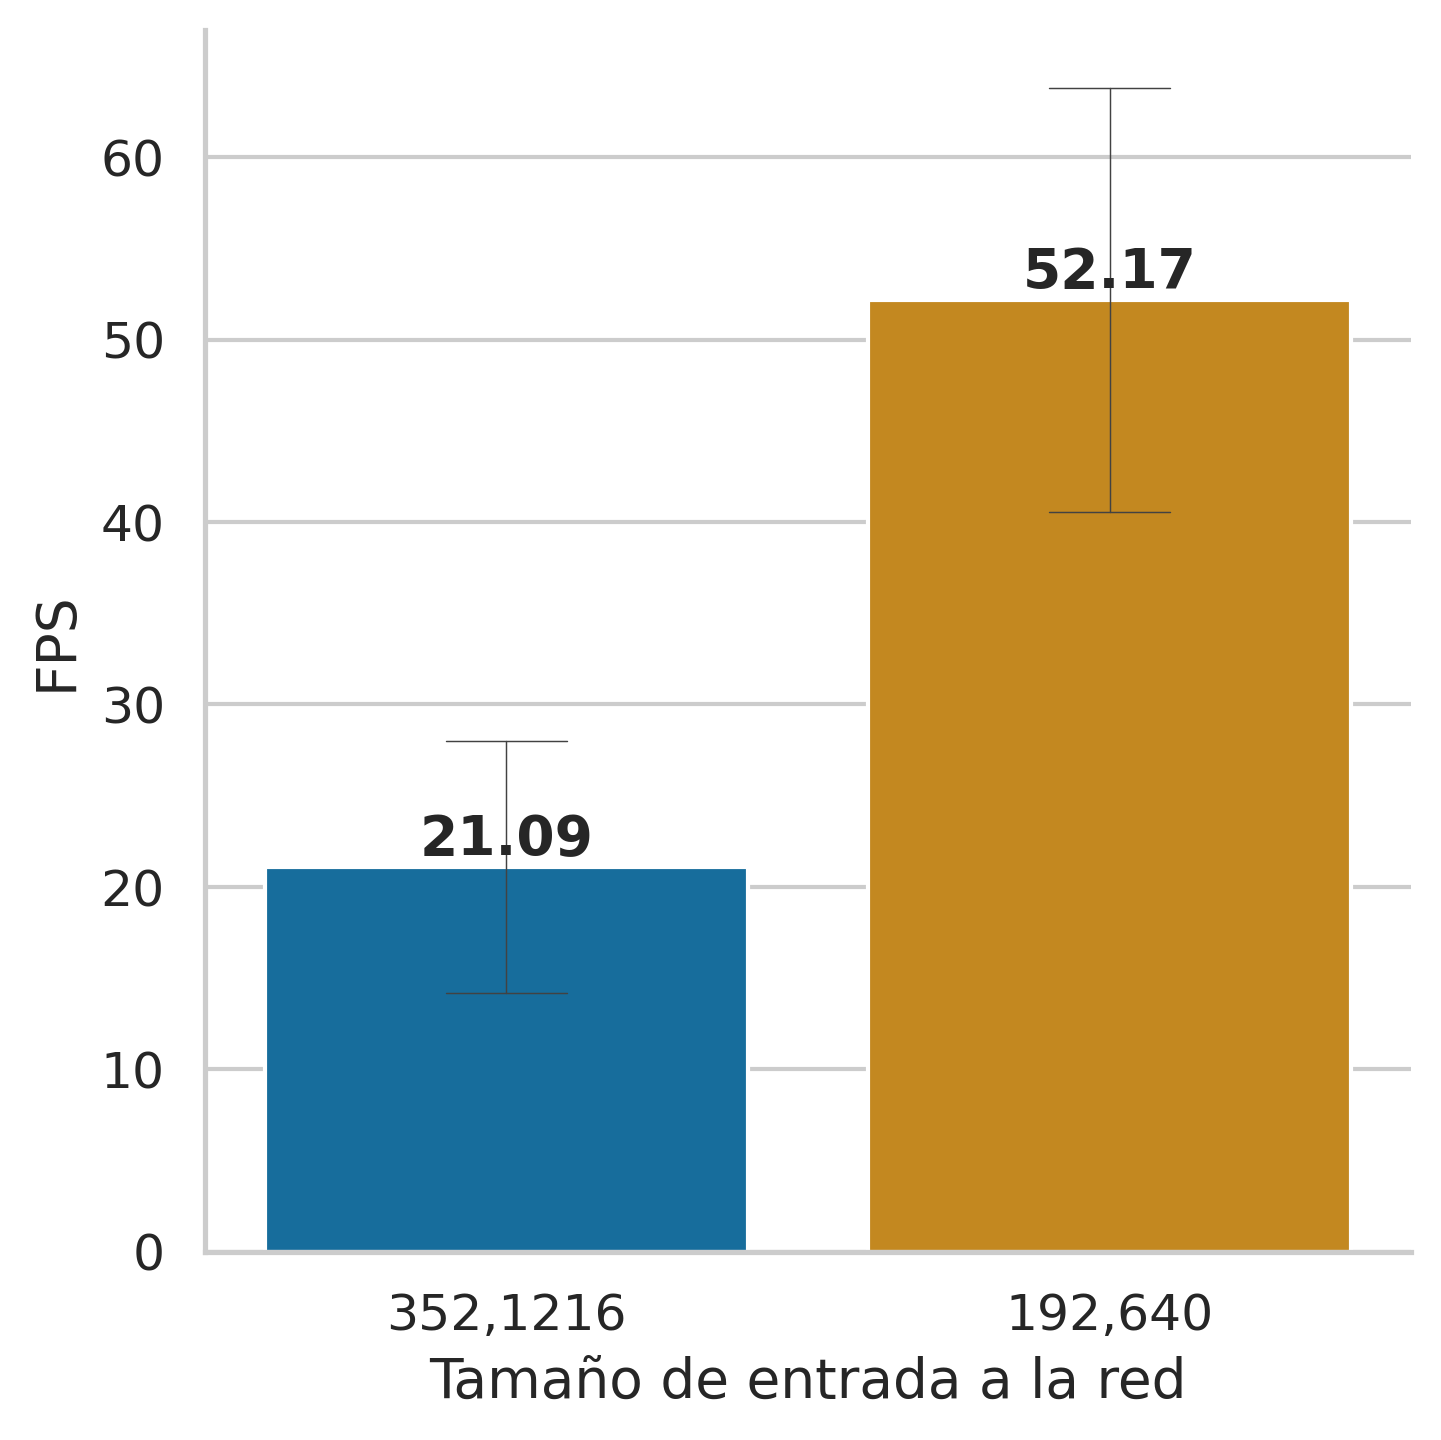
\includegraphics[width=0.95\linewidth]{imagenes/Resultados/velocidad_inferencia_entrada.png} 
\caption{FPS promedios de los modelos en función del tamaño de su entrada. Las barras grises representan la desviación estándar de las medidas.}
\label{fig:resultados-inf-tam-entrada}
\end{wrapfigure}

En cuanto a la medida de la velocidad de inferencia, que si que es posible obtener independientemente de que los pesos correspondan al modelo entrenado o no, en la Figura \ref{fig:resultados-inf-tam-entrada} se puede apreciar la diferencia en función del tamaño de entrada de los FPS medios de todas las modificaciones realizadas sobre el modelo DPT. El valor de la izquierda, corresponde al tamaño con el que se evalúa KITTI en la publicación original \cite{visiontransformerDPT}, mientras que el de la derecha es la reducción de tamaño establecida en este trabajo. Dado que este cambio es significativo y es, en términos de magnitud, el que mayor aceleración media conlleva ($\times2.47$), en las siguientes Figuras que representan los FPS en función de los otros cambios mencionados en la sección TODO se presentará la influencia de dichos cambios en la inferencia tanto con la entrada original como con la entrada reducida para poder así valorar también la mejora de rendimiento que conllevaría la modificación si no se hubiese modificado el tamaño de la entrada.

\subsubsection{Número de cabezas}

\todo[inline]{Completar el párrafo de abajo cuando estén los resultados de las otras métricas, a lo mejor algo de la explicación de los resultados llevarlo a un apartado de discusión?}

Respecto de la influencia de este parámetro en la velocidad de inferencia, en la Figura \ref{fig:resultados-inf-num-cabezas} se puede observar, agrupado por tamaño de entrada, backbone, y número de cabezas, los promedios de los FPS de los modelos. Teniendo en cuenta que las capas de atención del modelo original tienen 12 cabezas, era de esperar que aquellos modelos con una sola cabeza fueran más rápidos y los que cuentan con 24 fuesen más lentos. Además, este cambio en la velocidad de inferencia relativa es mayor en el caso de la entrada sin escalar que en el caso de la entrada escalada. Por ejemplo, en el paso de 12 a una cabeza con la entrada sin escalar, el incremento en el número de FPS es de $\times1.2$ y $\times1.26$ dependiendo del backbone empleado, mientras que al escalar la salida este cambio pasa a ser $\times1.04$ y $\times1.03$ respectivamente. Esto se debe a la implementación previamente comentada en la sección TODO, ya que TODO reescribir esto
\begin{figure}[H]
\centering
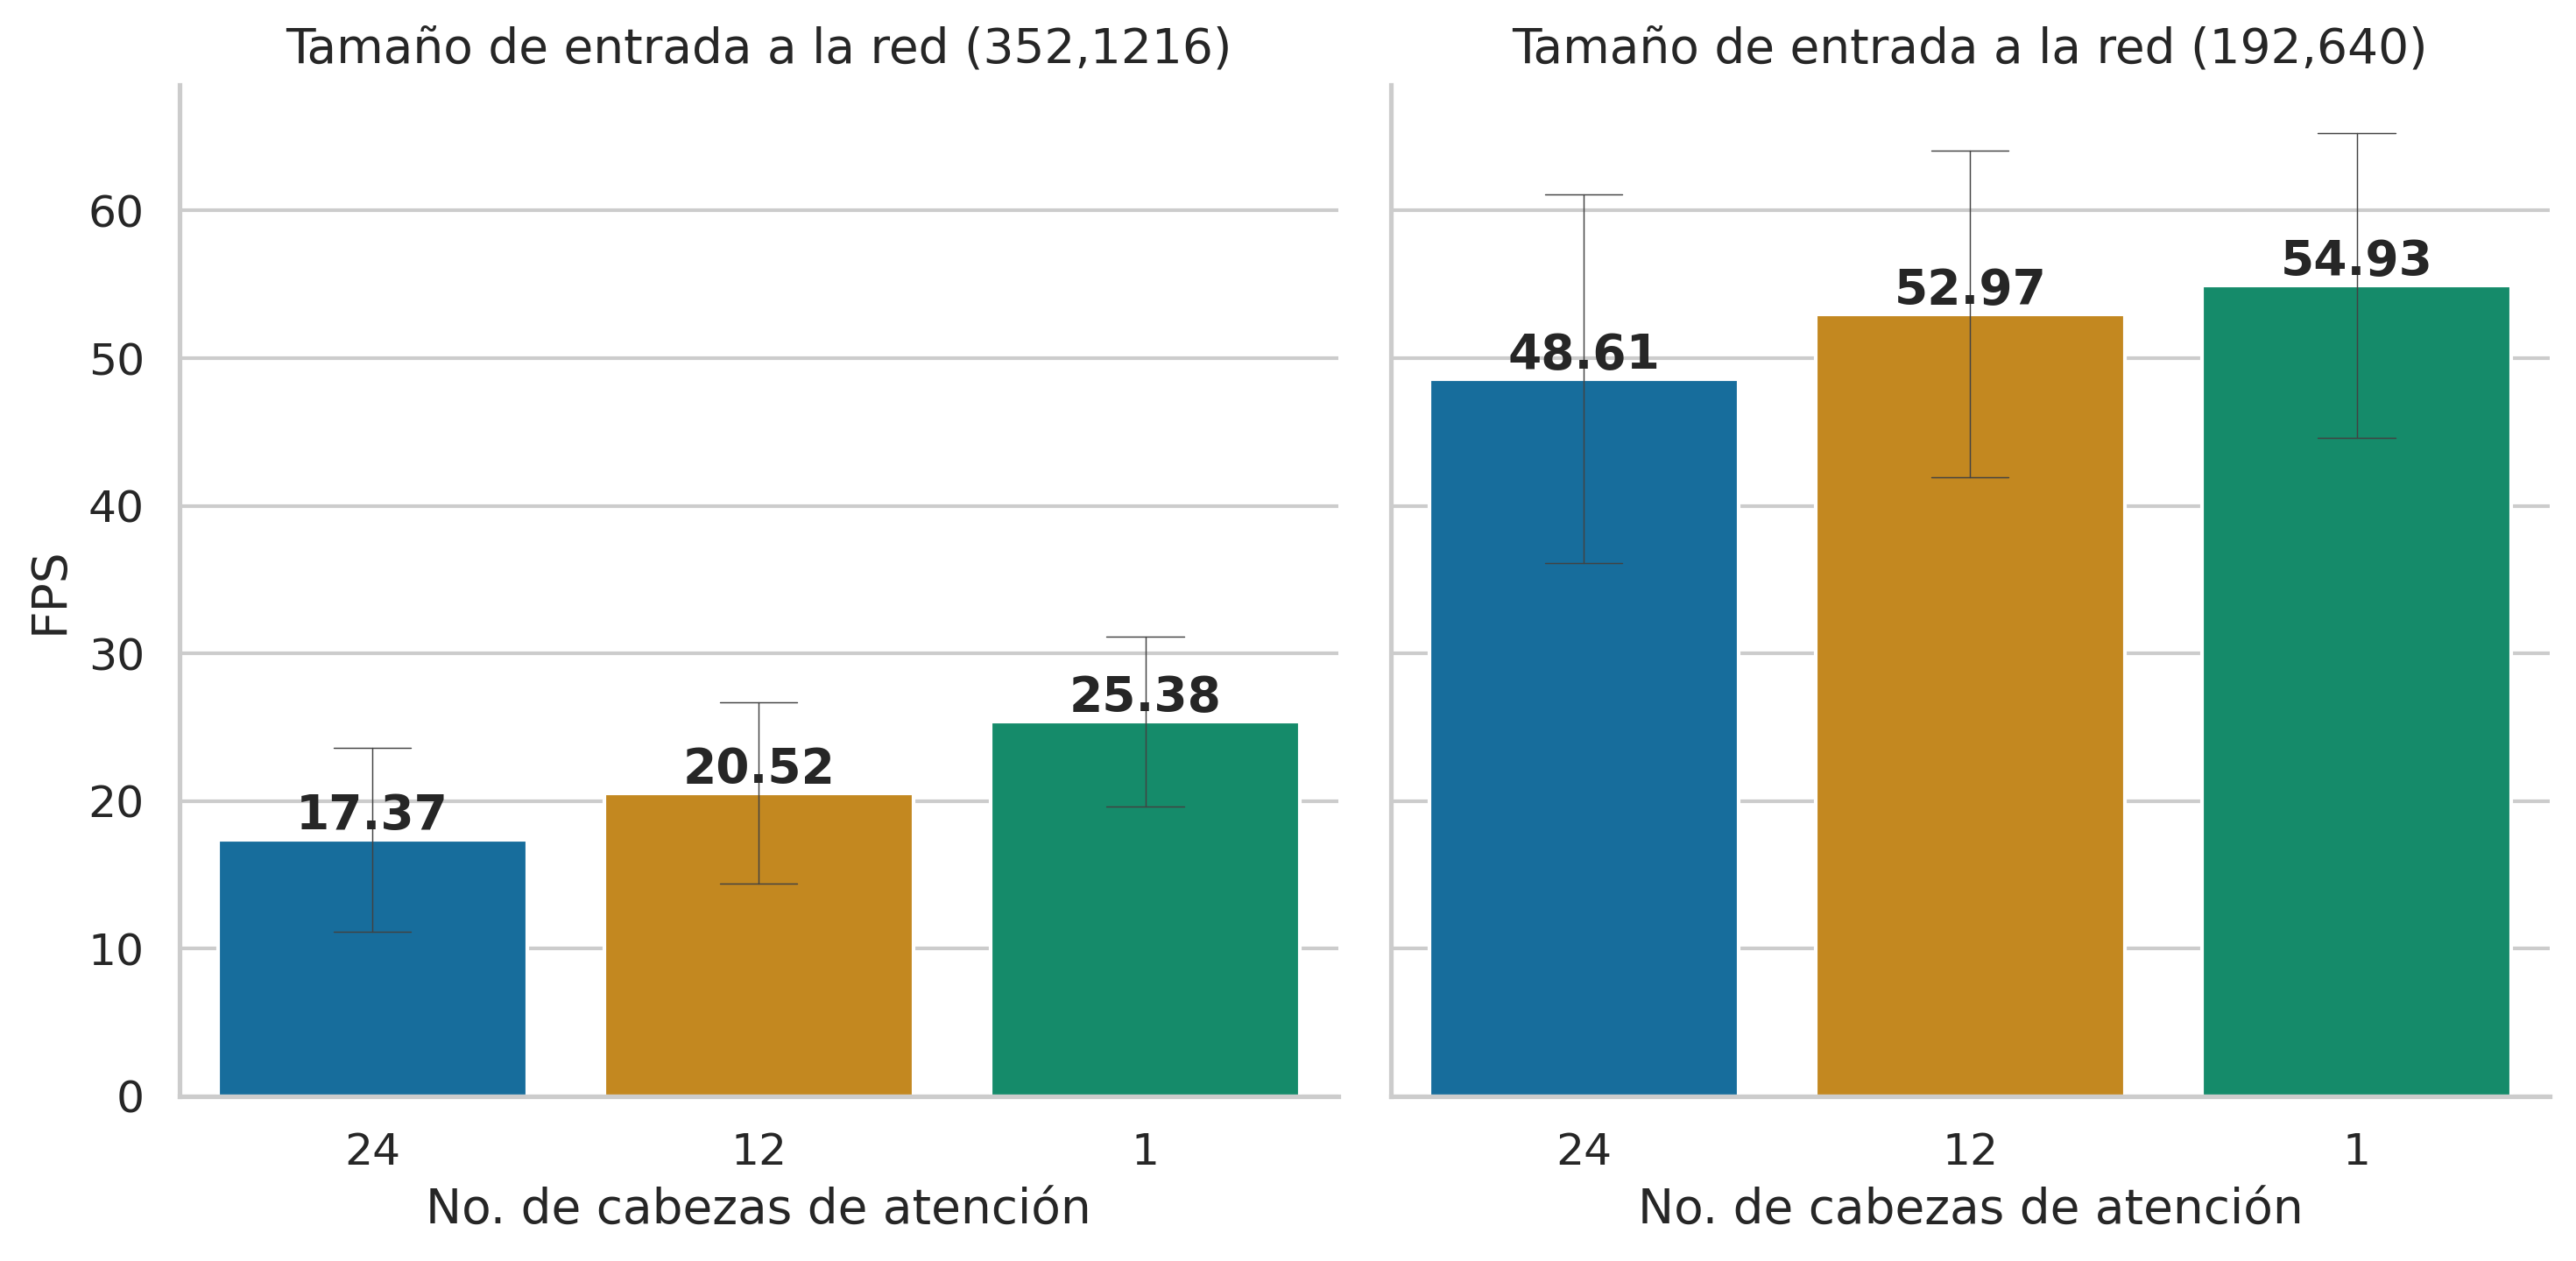
\includegraphics[width=0.9\linewidth]{imagenes/Resultados/velocidad_inferencia_cabezas_atencion.png} 
\captionsetup{width=.8\linewidth}
\caption{Resultados de.}
\label{fig:resultados-inf-num-cabezas}
\end{figure}

\subsubsection{Capas de atención eficiente}

\begin{figure}[H]
\centering
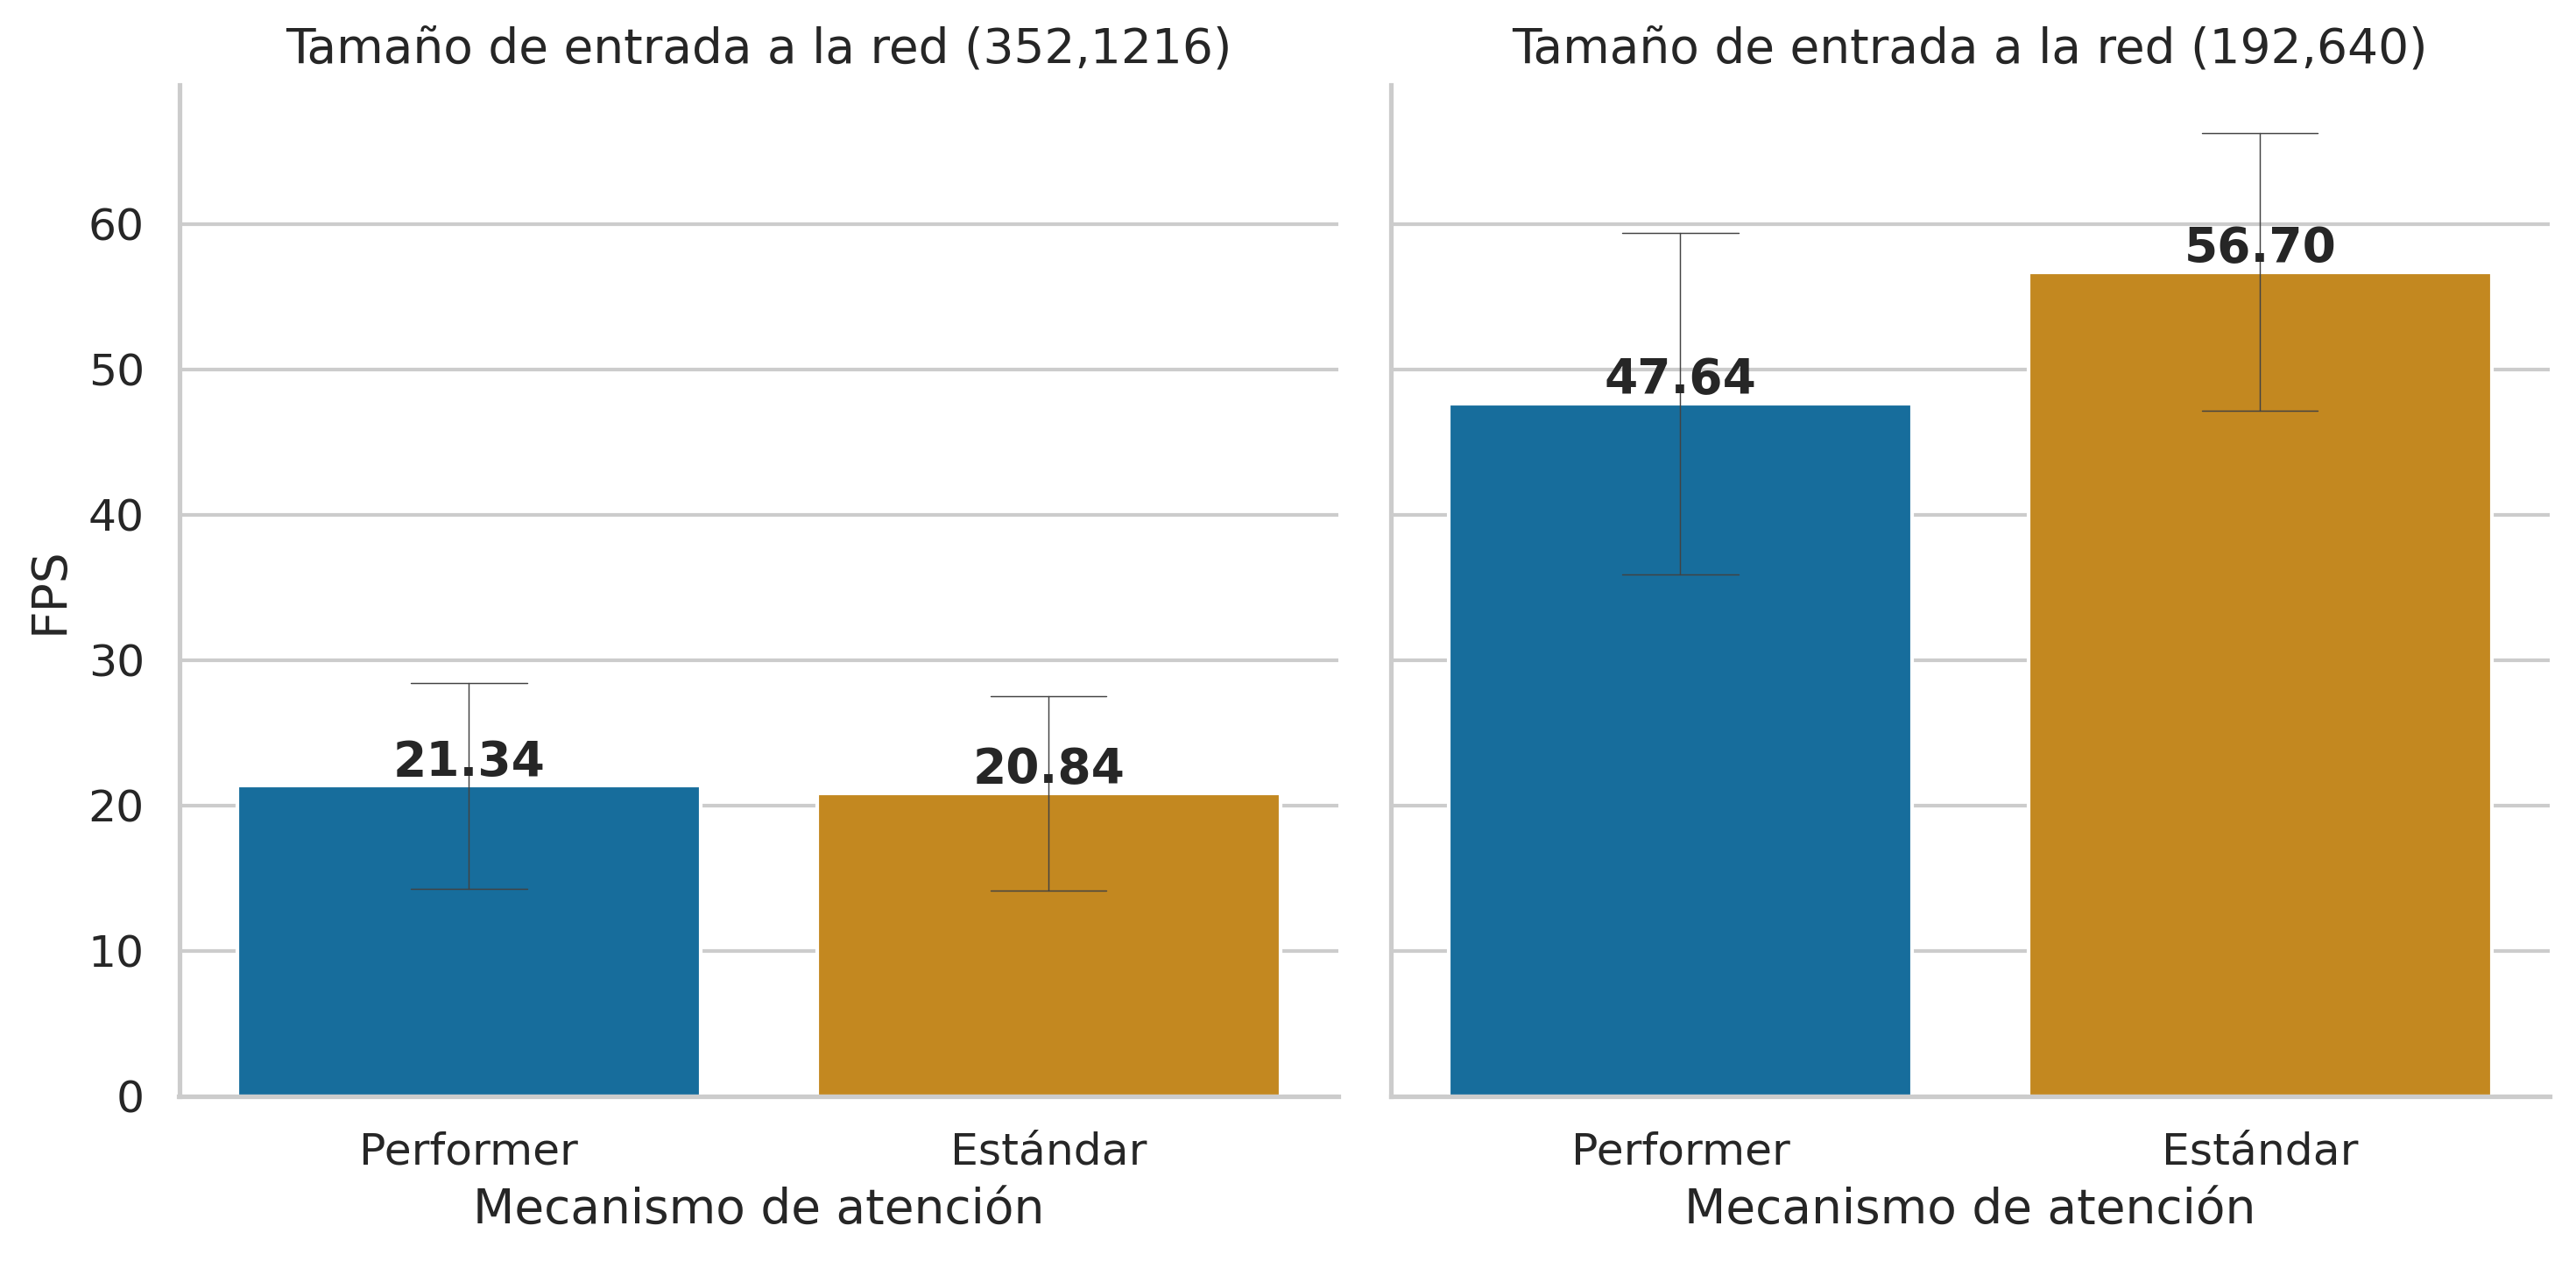
\includegraphics[width=0.9\linewidth]{imagenes/Resultados/velocidad_inferencia_mecanismo_atencion.png} 
\captionsetup{width=.8\linewidth}
\caption{Resultados de.}
\label{fig:resultados-inf-mec-atention}
\end{figure}

\begin{figure}[H]
\centering
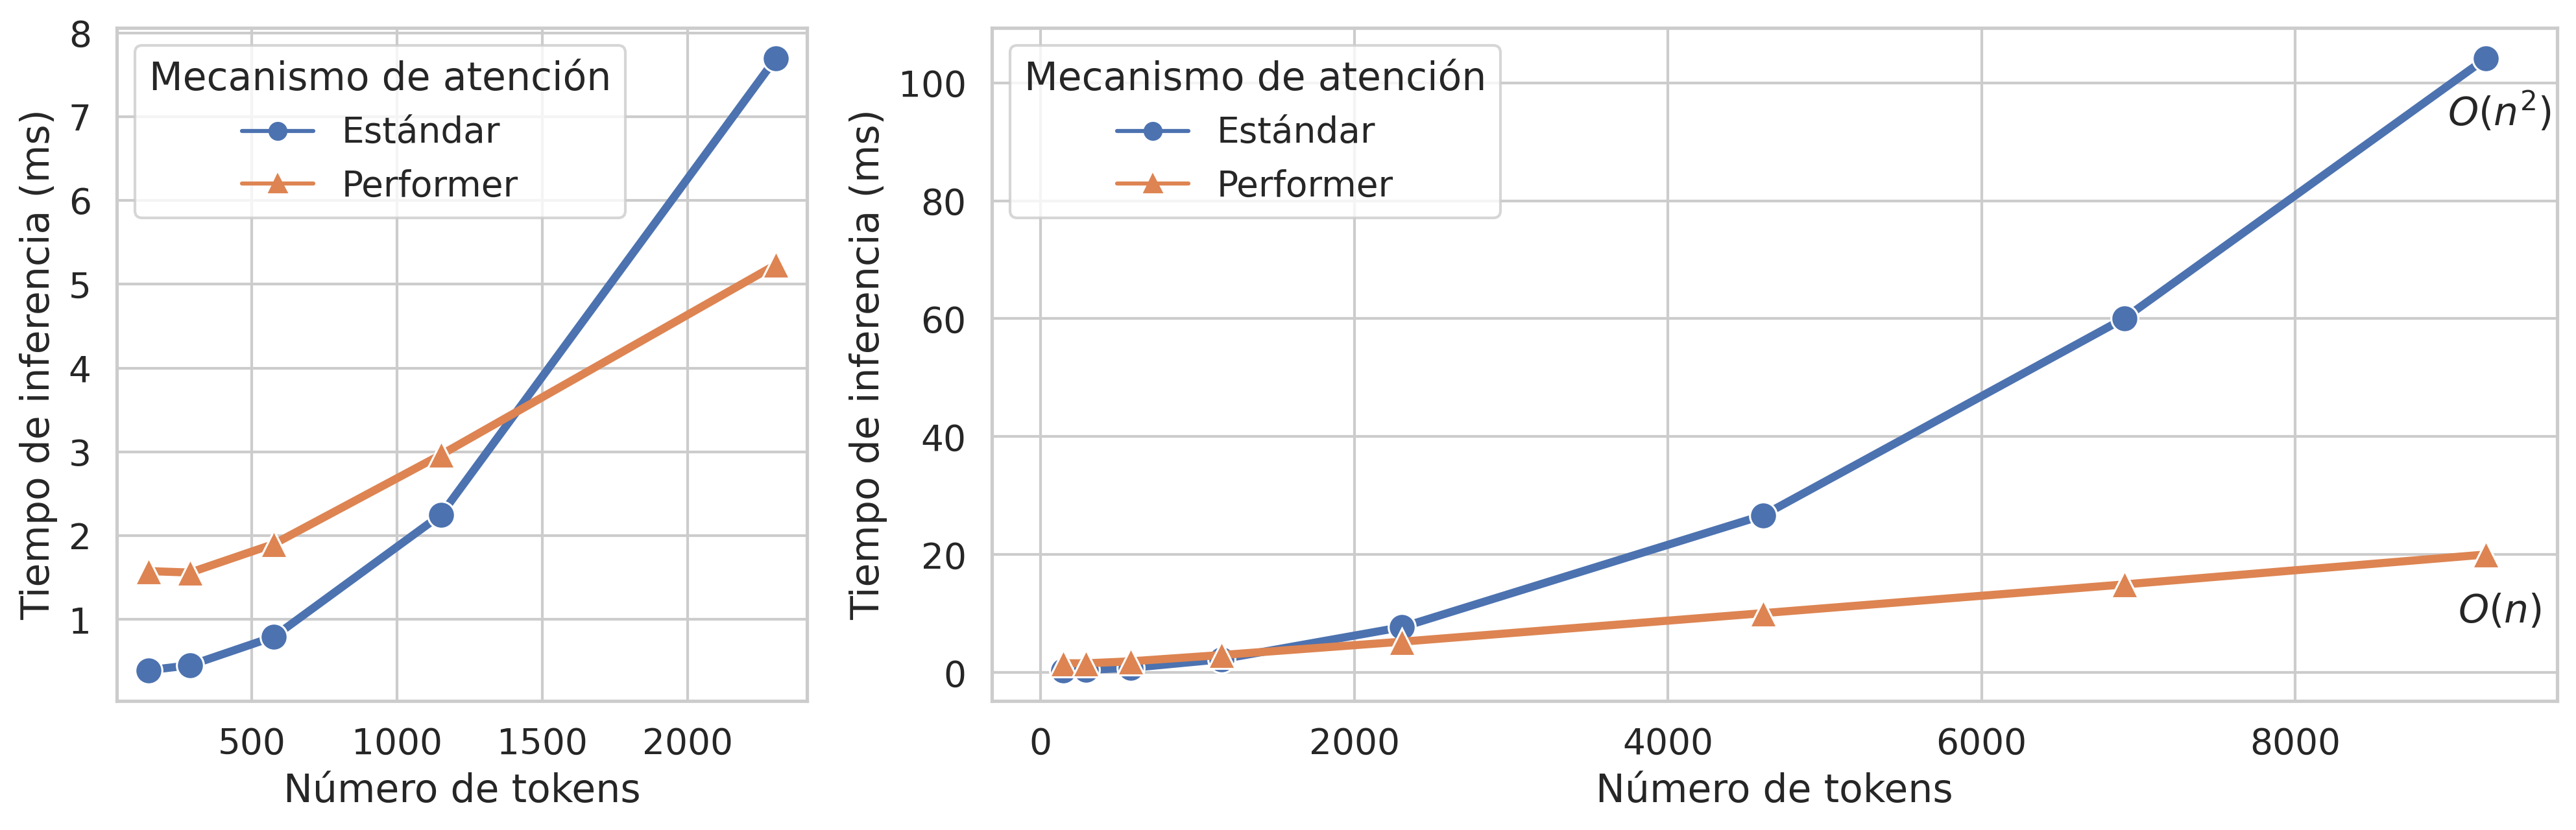
\includegraphics[width=\linewidth]{imagenes/Resultados/complejidad_mecanismo_atencion.png} 
\captionsetup{width=.8\linewidth}
\caption{Resultados de.}
\label{fig:resultados-complejidad-mec-atencion}
\end{figure}

\subsubsection{Cambio en los hooks del transformer y eliminación de las capas de atención posteriores}

\begin{figure}[H]
\centering
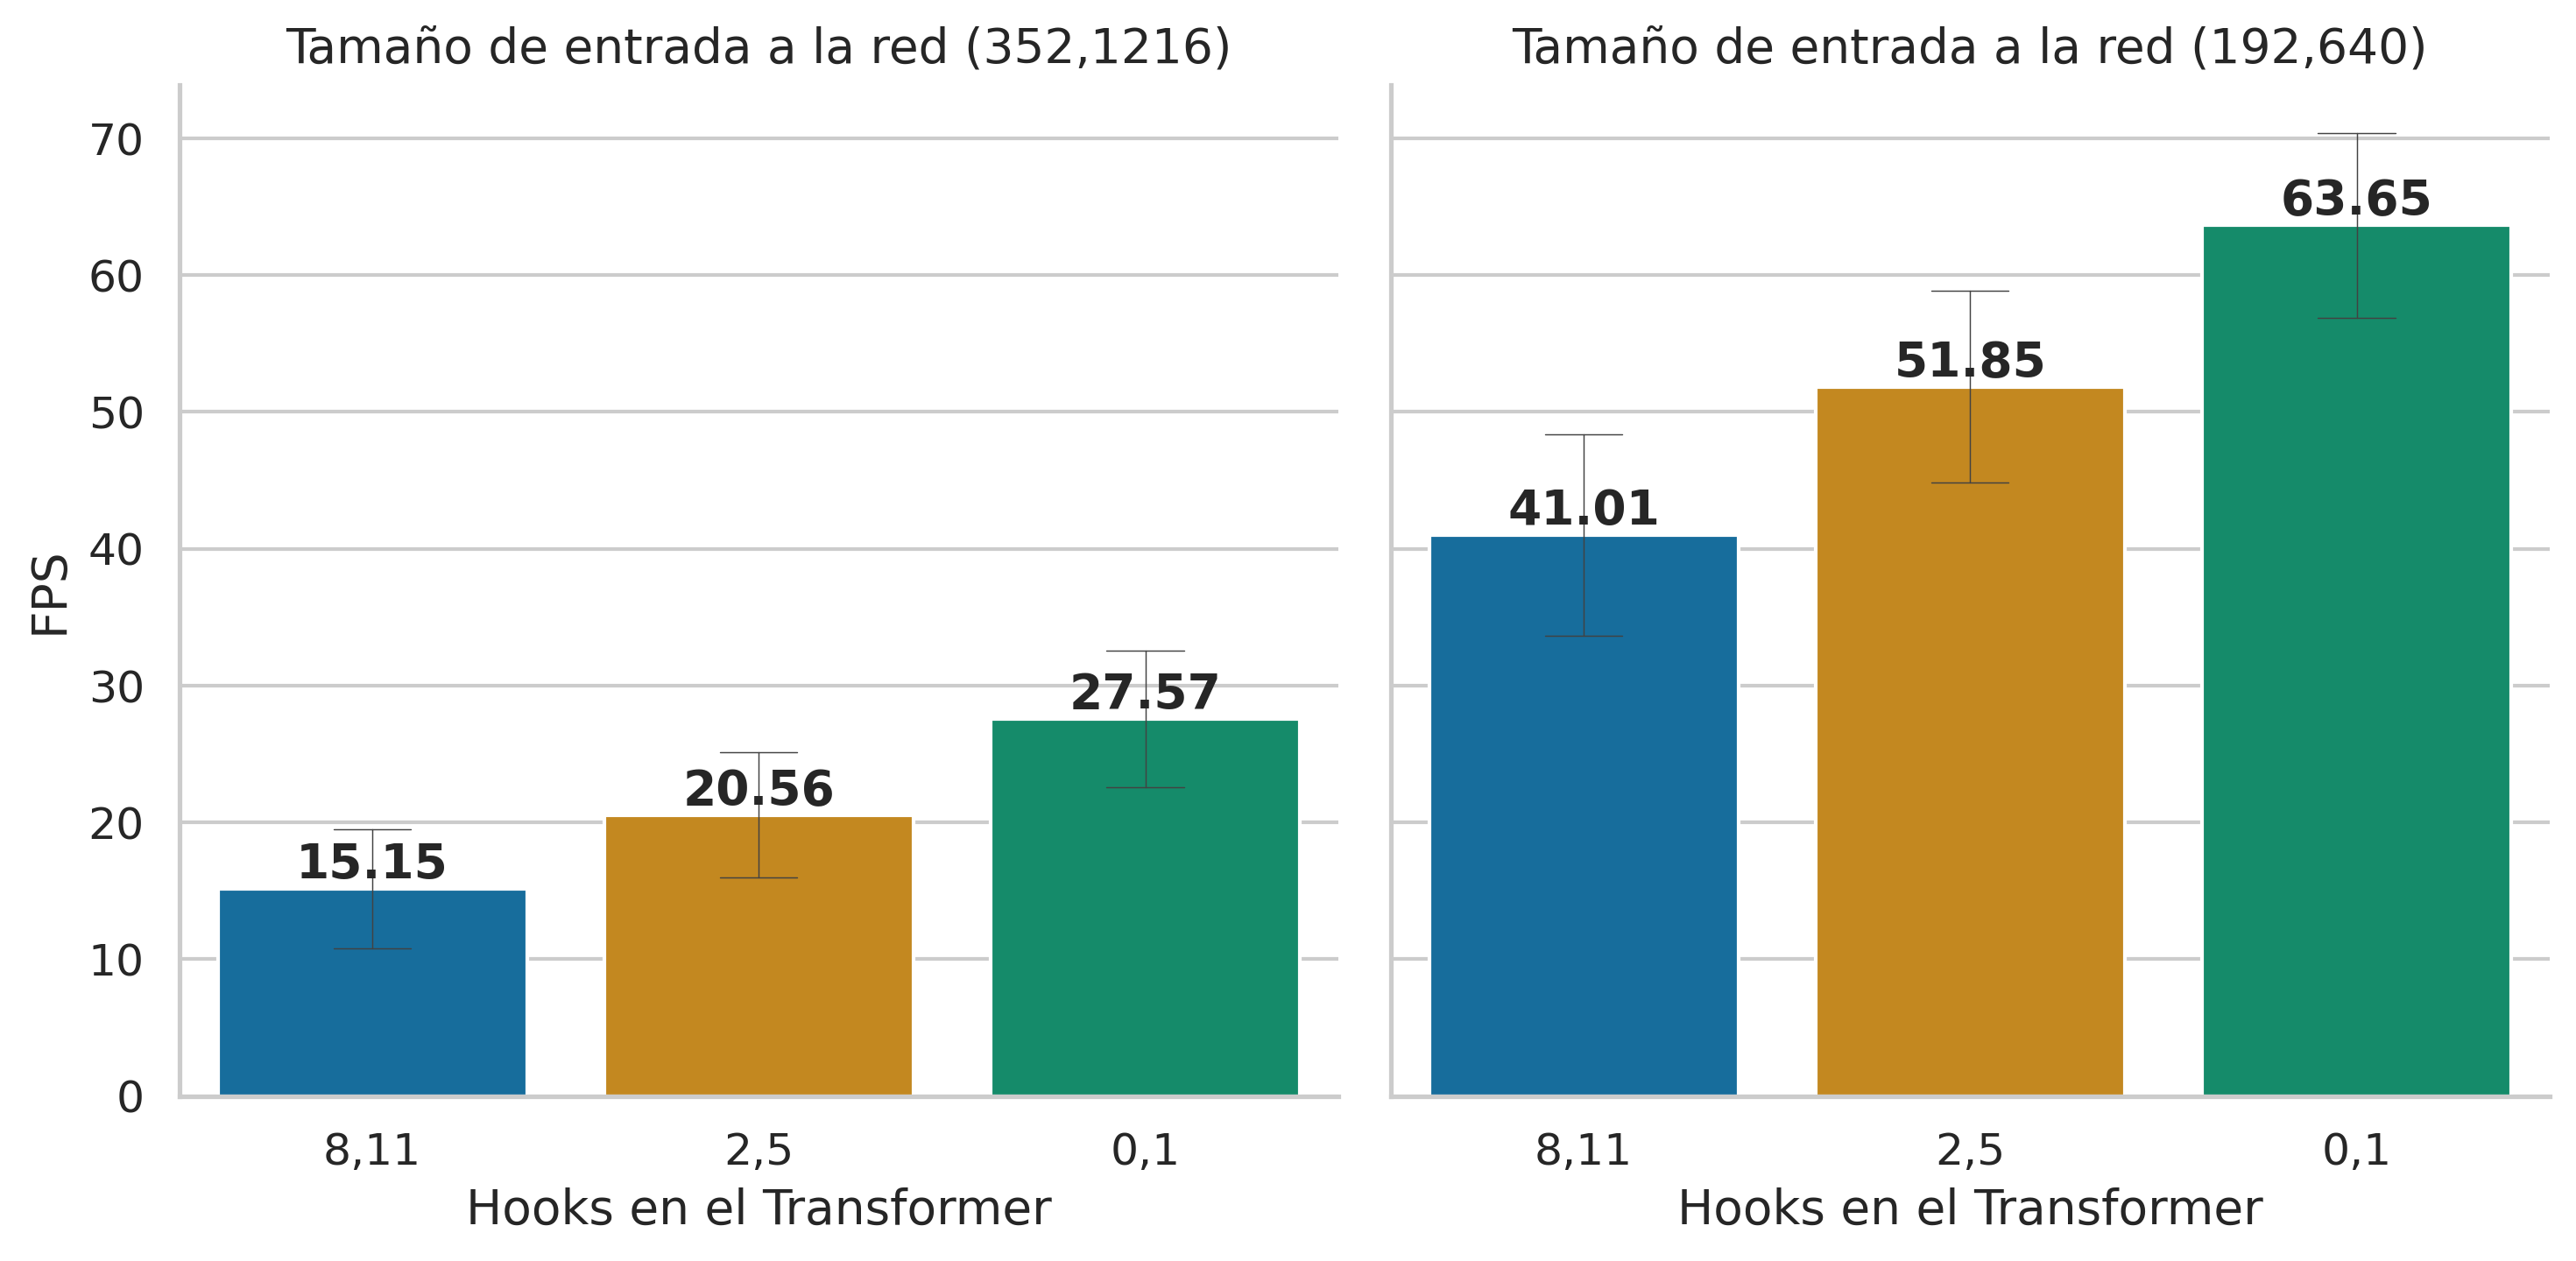
\includegraphics[width=0.9\linewidth]{imagenes/Resultados/velocidad_inferencia_hooks.png} 
\captionsetup{width=.8\linewidth}
\caption{Resultados de.}
\label{fig:resultados-inf-hooks}
\end{figure}

\subsubsection{Cambio del backbone convolucional}

\todo[inline]{Comparar los feature maps que saca uno y otro?}
\todo[inline]{Justificar que al no estar preentrenado en mix6 los resultados son peores con un entrenamiento de un resnet a partir de imagenet}

\begin{figure}[H]
\centering
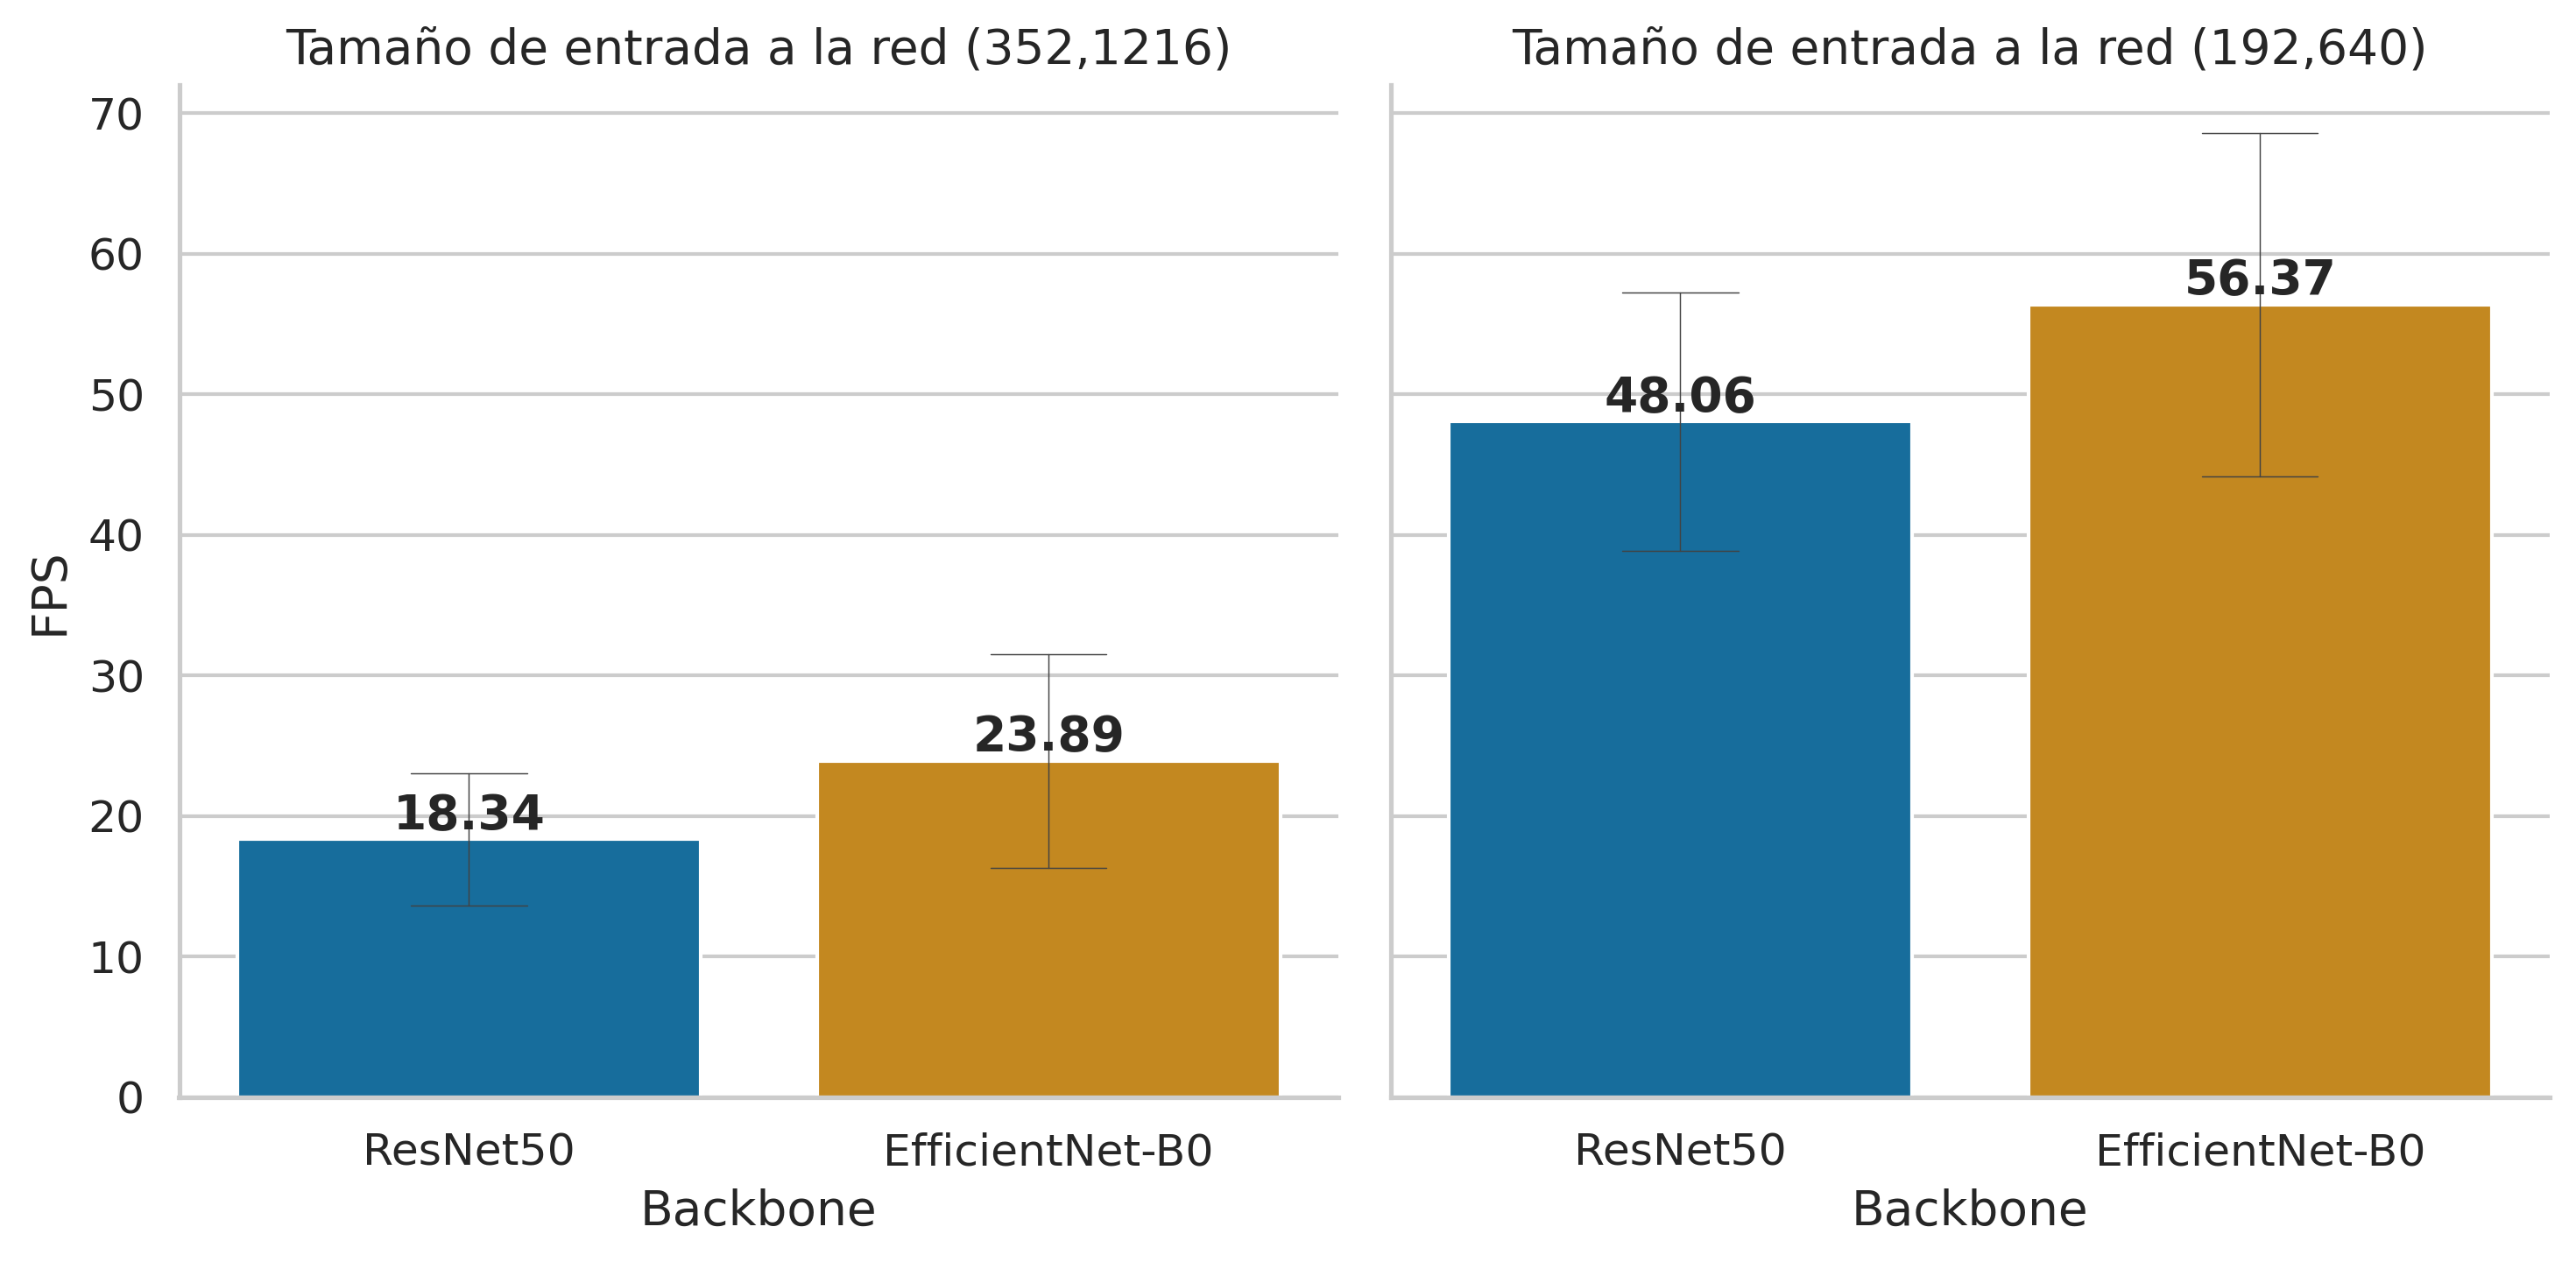
\includegraphics[width=0.9\linewidth]{imagenes/Resultados/velocidad_inferencia_backbone.png} 
\captionsetup{width=.8\linewidth}
\caption{Resultados de.}
\label{fig:resultados-inf-backbone}
\end{figure}

\subsection{Resultados cualitativos}

%% http://www.peteryu.ca/tutorials/publishing/latex_captions_old
%% https://tex.stackexchange.com/questions/162824/vertical-spacing-between-subfloat
%% https://tex.stackexchange.com/questions/395515/how-to-scale-and-align-figures-and-tables-in-latex-in-a-3x2-grid-like-manner
\captionsetup[subfigure]{labelformat=empty}
    \begin{figure}[!ht]
\centering
    \subfloat{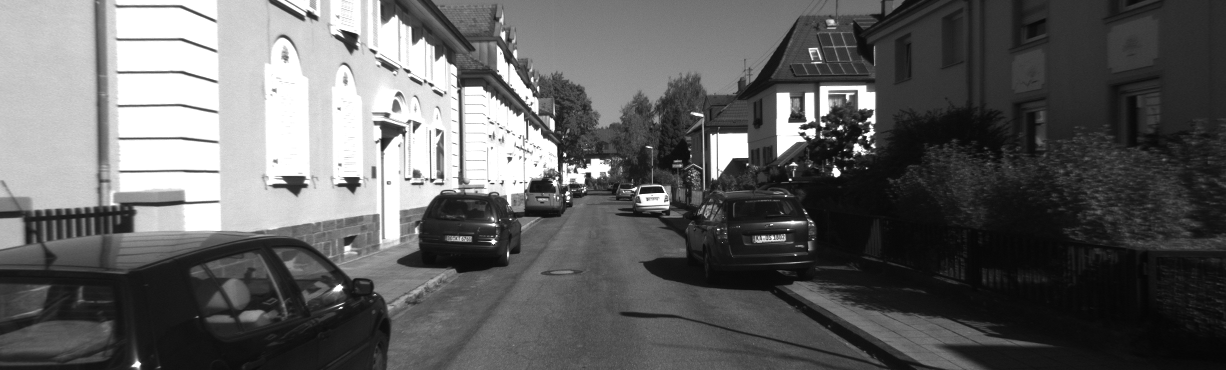
\includegraphics[width=0.33\linewidth]{imagenes/67_img0.png}}
\hfil
    \subfloat{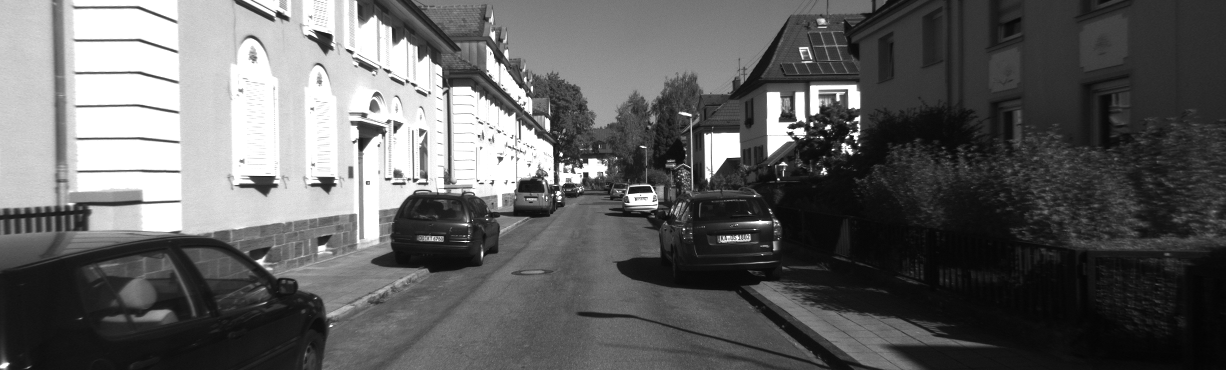
\includegraphics[width=0.33\linewidth]{imagenes/67_img1.png}}
\hfil
    \subfloat{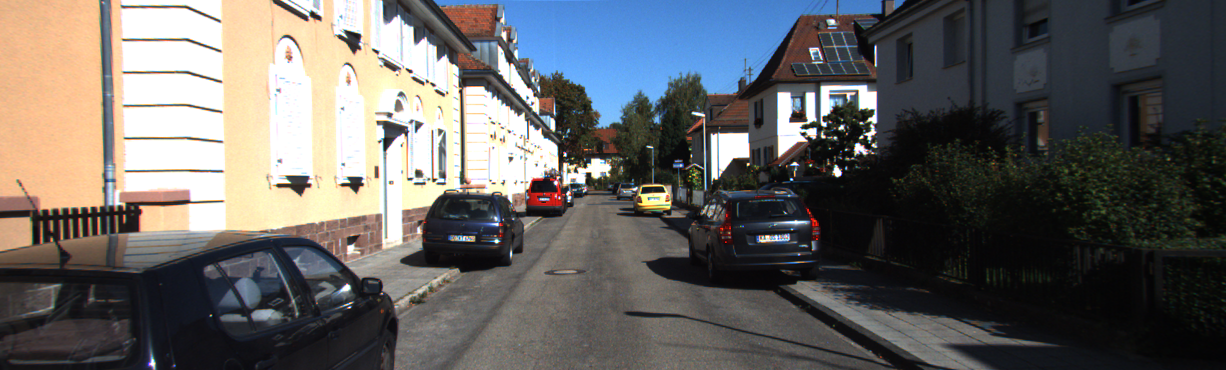
\includegraphics[width=0.33\linewidth]{imagenes/67_img2.png}}\\[-2ex]

    \subfloat{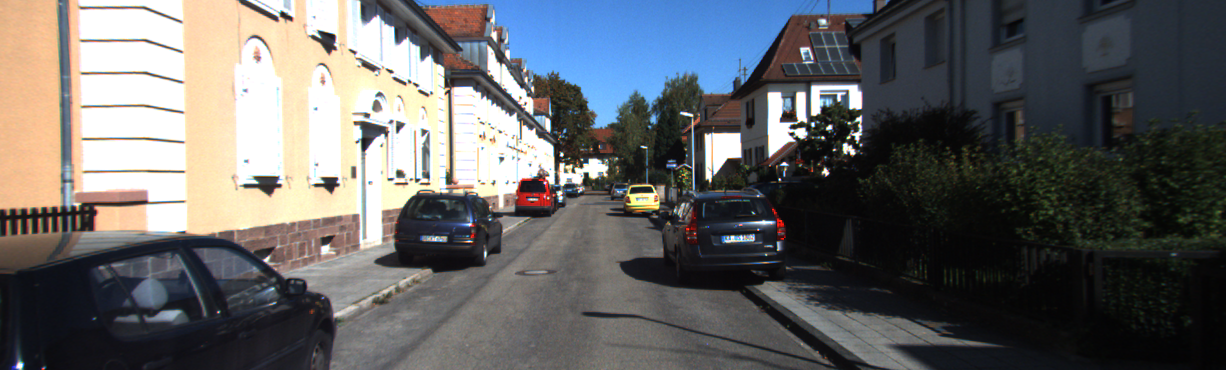
\includegraphics[width=0.33\linewidth]{imagenes/67_img3.png}}
\hfil
    \subfloat{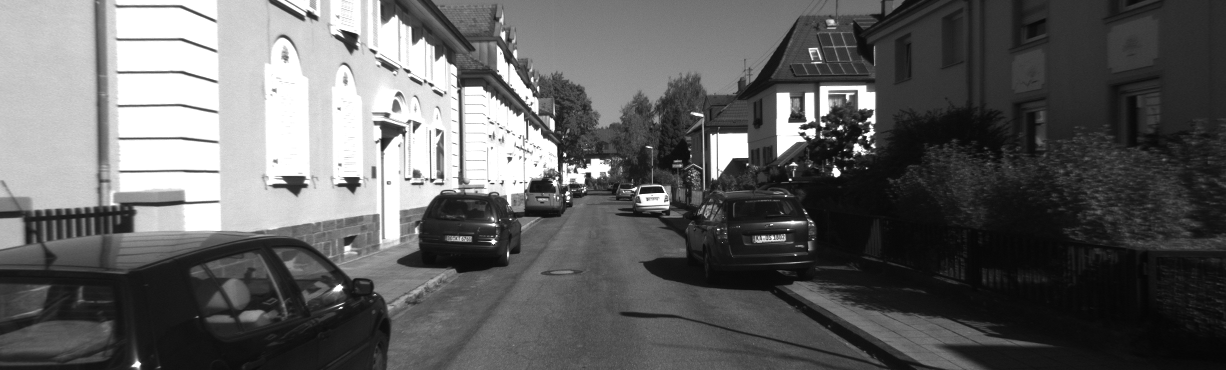
\includegraphics[width=0.33\linewidth]{imagenes/67_img0.png}}
\hfil
    \subfloat{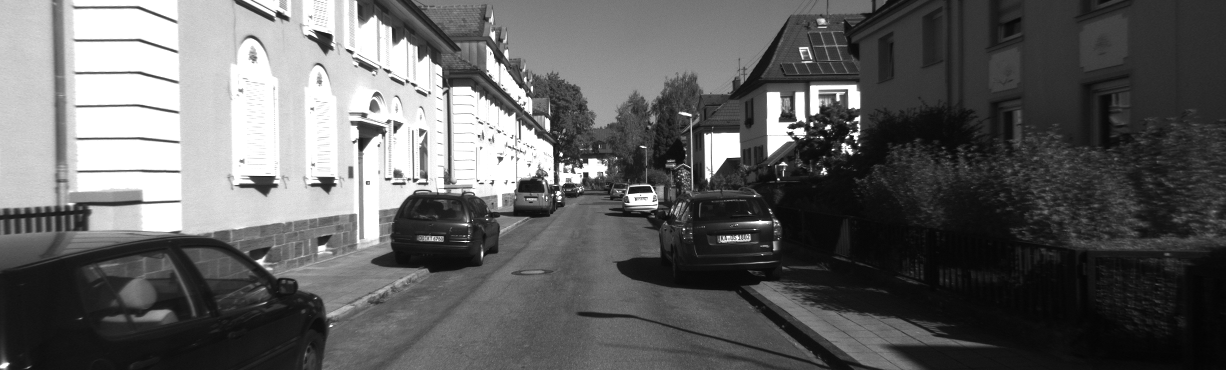
\includegraphics[width=0.33\linewidth]{imagenes/67_img1.png}}\\[-2ex]
    
    \subfloat{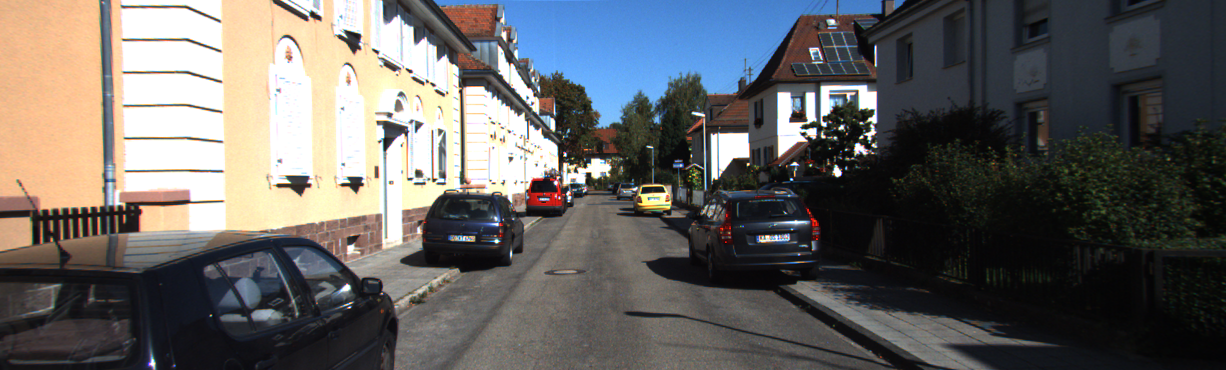
\includegraphics[width=0.33\linewidth]{imagenes/67_img2.png}}
\hfil
    \subfloat{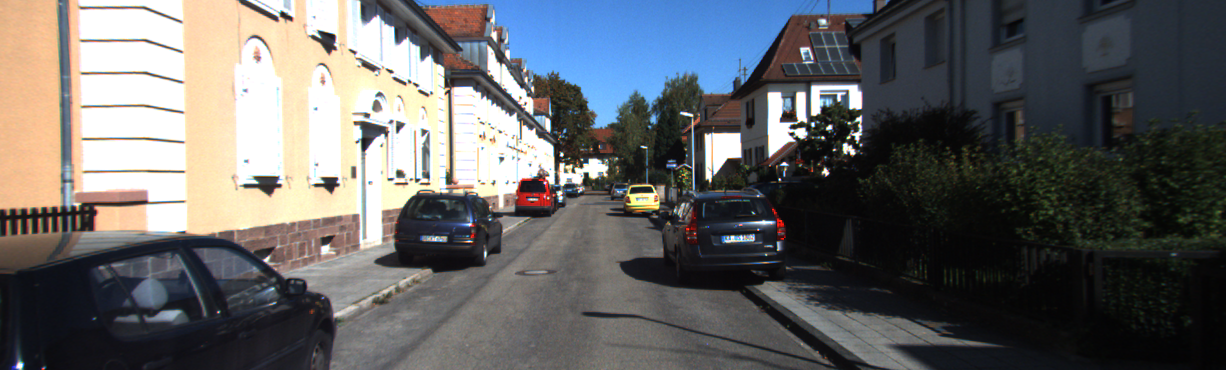
\includegraphics[width=0.33\linewidth]{imagenes/67_img3.png}}
\hfil
    \subfloat{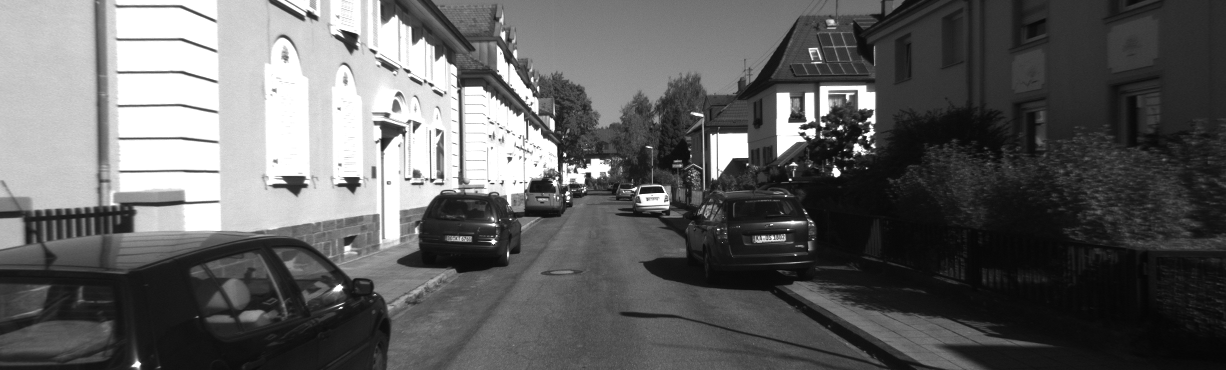
\includegraphics[width=0.33\linewidth]{imagenes/67_img0.png}}\\[-2ex]
    
    \subfloat{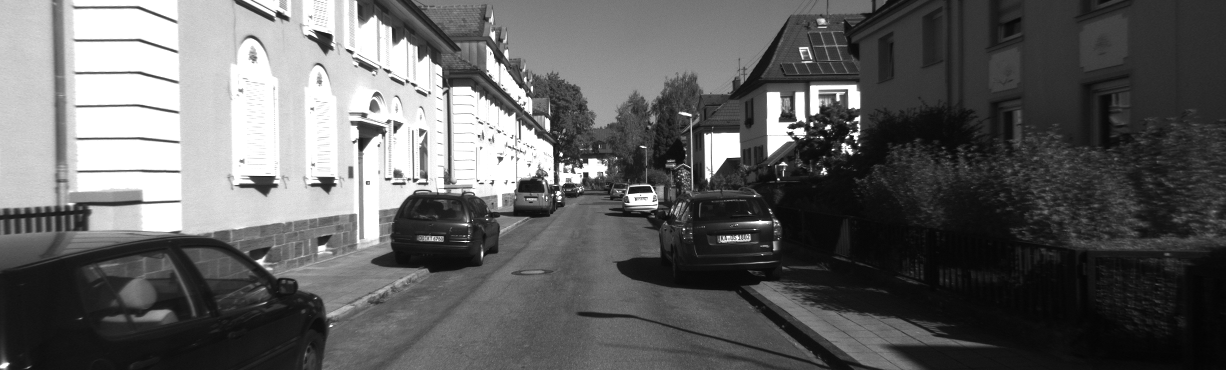
\includegraphics[width=0.33\linewidth]{imagenes/67_img1.png}}
\hfil
    \subfloat{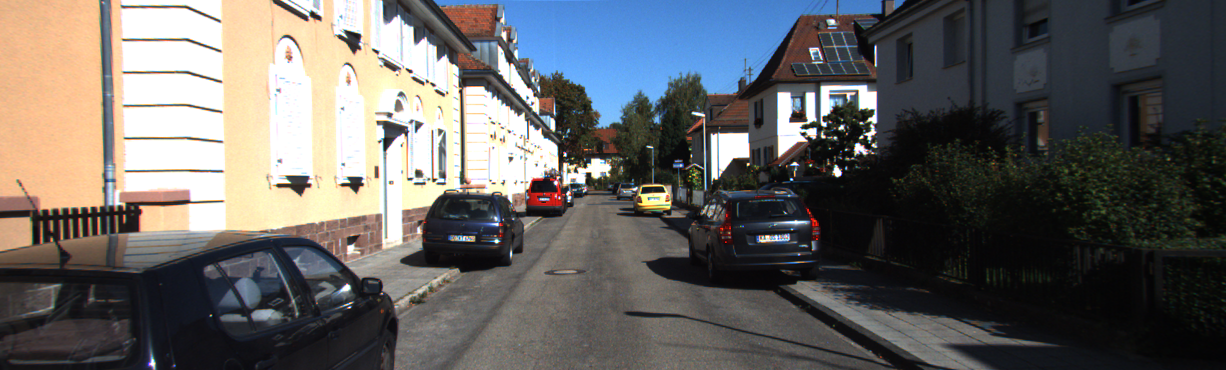
\includegraphics[width=0.33\linewidth]{imagenes/67_img2.png}}
\hfil
    \subfloat{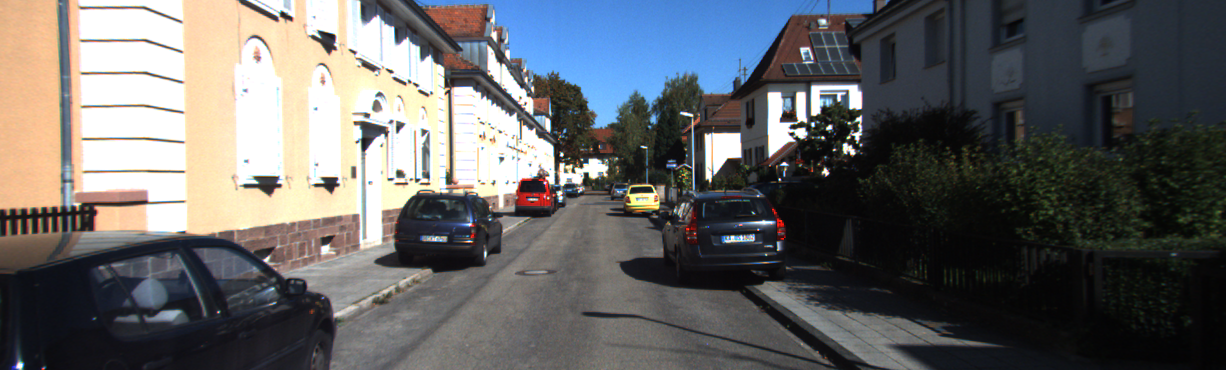
\includegraphics[width=0.33\linewidth]{imagenes/67_img3.png}}\\[-2ex]
    
    \subfloat{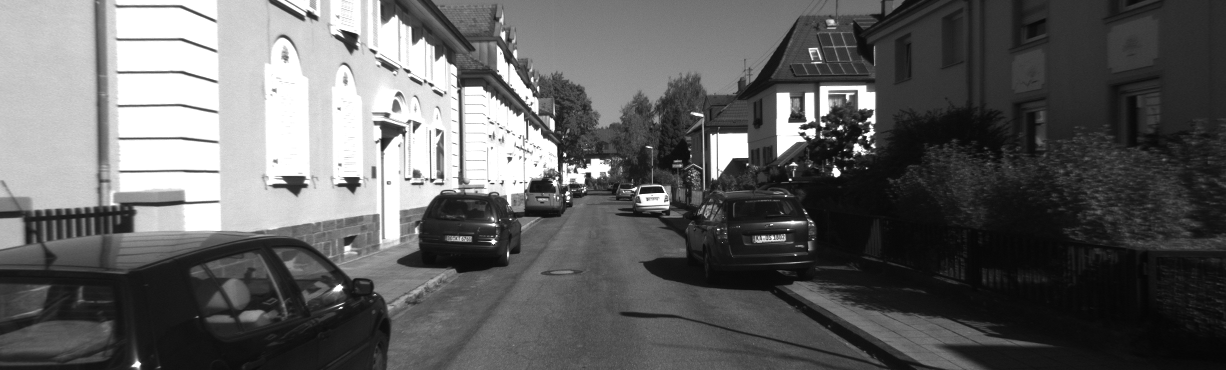
\includegraphics[width=0.33\linewidth]{imagenes/67_img0.png}}
\hfil
    \subfloat{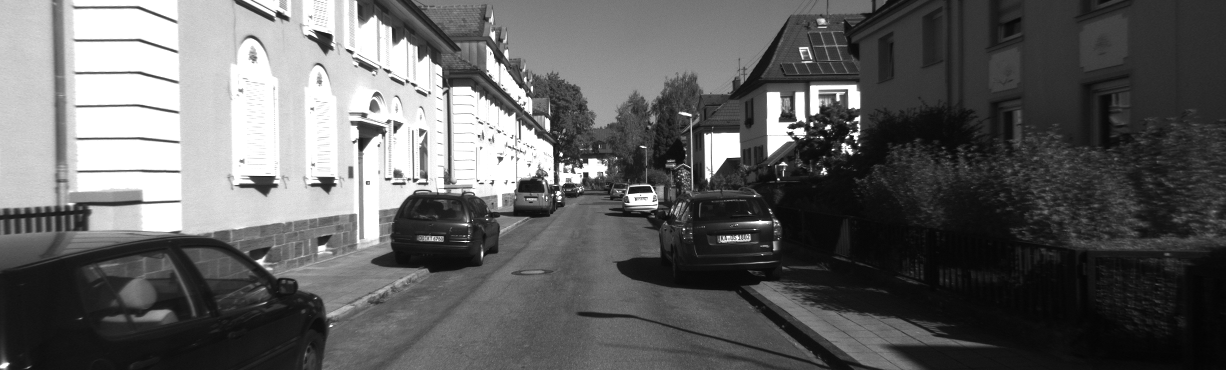
\includegraphics[width=0.33\linewidth]{imagenes/67_img1.png}}
\hfil
    \subfloat{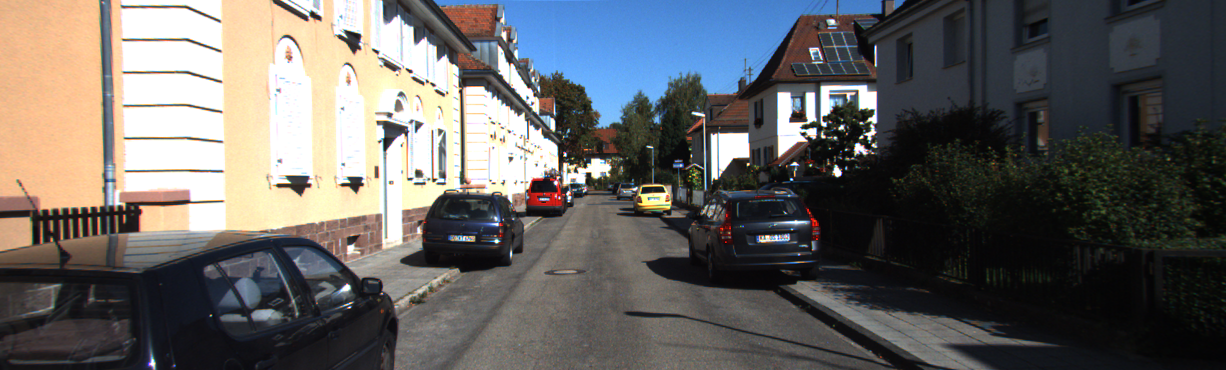
\includegraphics[width=0.33\linewidth]{imagenes/67_img2.png}}\\[-2ex]

    \subfloat{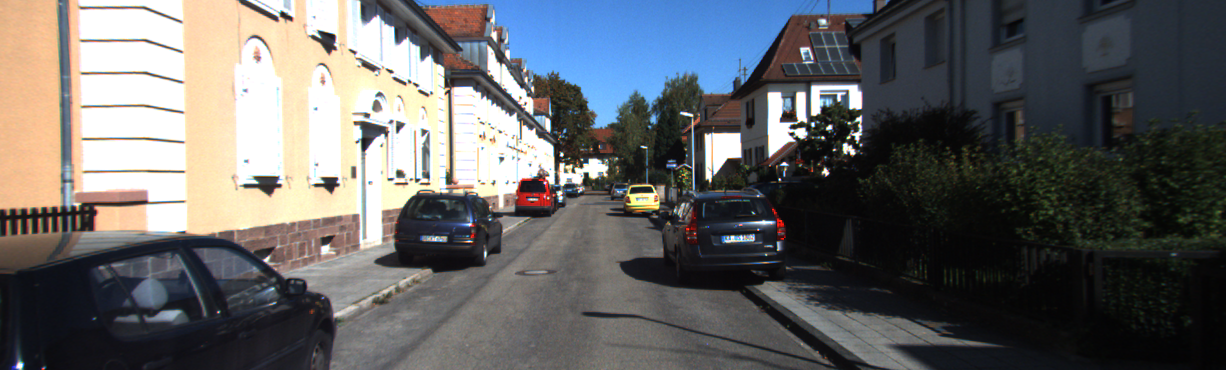
\includegraphics[width=0.33\linewidth]{imagenes/67_img3.png}}
\hfil
    \subfloat{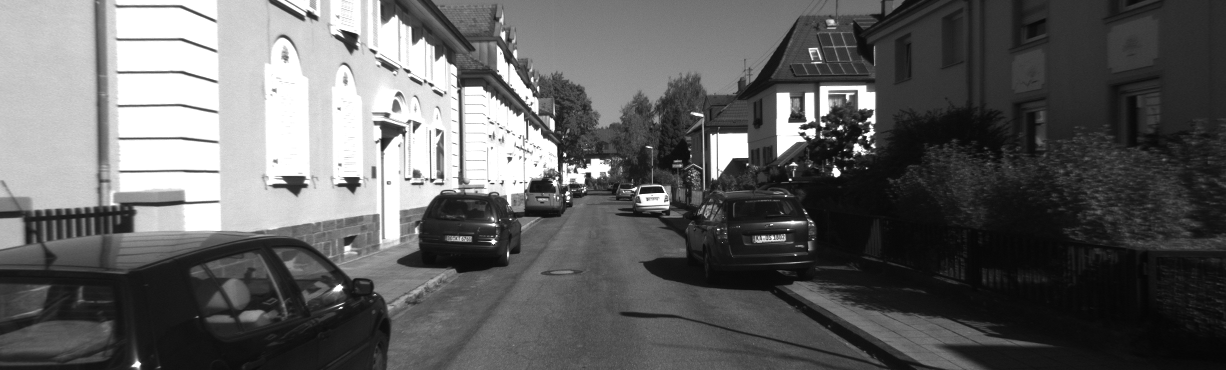
\includegraphics[width=0.33\linewidth]{imagenes/67_img0.png}}
\hfil
    \subfloat{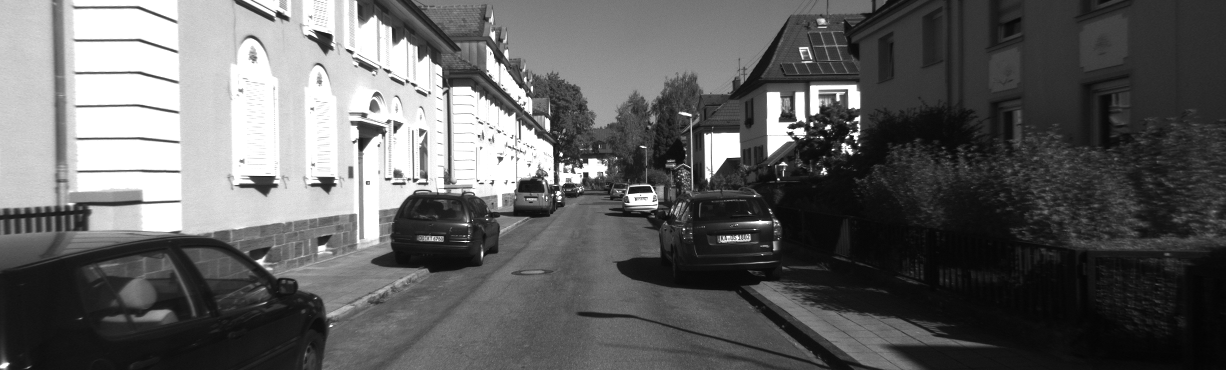
\includegraphics[width=0.33\linewidth]{imagenes/67_img1.png}}\\[-2ex]
    
    \subfloat[Entrada]{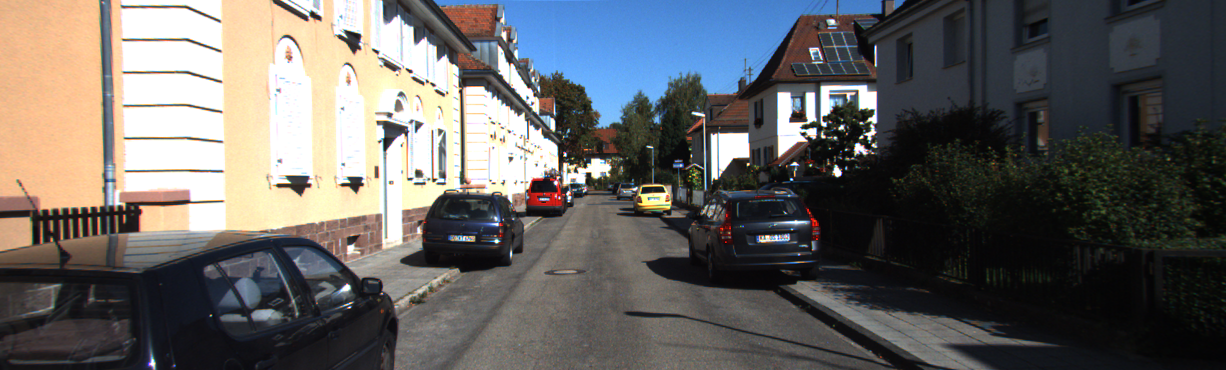
\includegraphics[width=0.33\linewidth]{imagenes/67_img2.png}}
\hfil
    \subfloat[Salida DPT modificado]{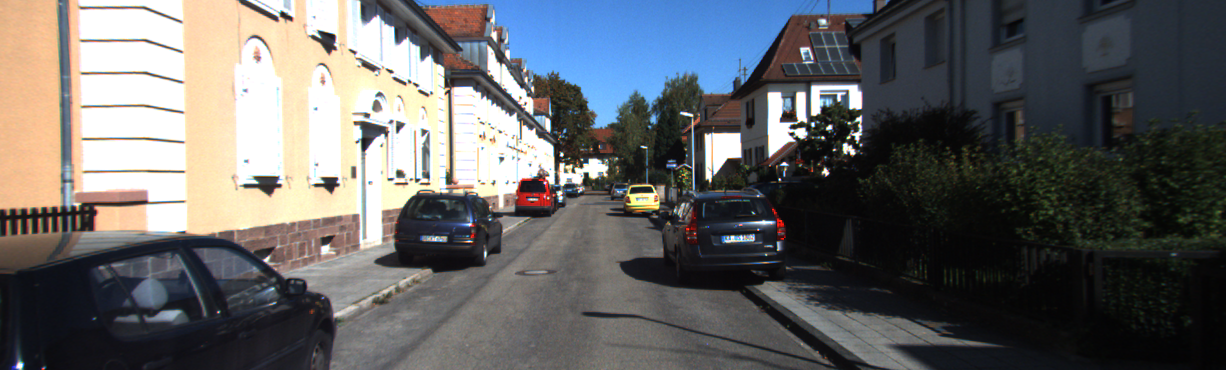
\includegraphics[width=0.33\linewidth]{imagenes/67_img3.png}}
\hfil
    \subfloat[Salida DPT sin modificar]{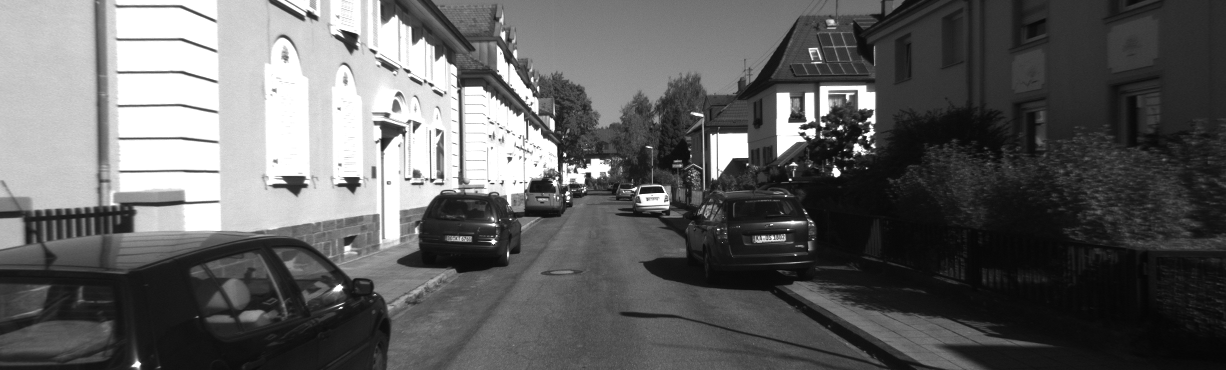
\includegraphics[width=0.33\linewidth]{imagenes/67_img0.png}}
    
\caption{Comparación cualitativa de resultados en el conjunto de evaluación entre el modelo DPT original y el modelo DPT con las modificaciones desarrolladas en este trabajo. Para facilitar su visualización, el rango de las profundidades predichas se ha ajustado a toda la escala de grises.}
    \label{fig:comparacion-cualitativa}
    \end{figure}
\captionsetup[subfigure]{labelformat=parens}

\clearpage

% Este ha sido principalmente un trabajo de revisión bibliográfica, cuyo objetivo era construir una base de conocimiento sobre la estimación de profundidades en imágenes monoculares con un cierto enfoque en las técnicas (tanto generales como específicas) capaces de acelerar dichos modelos. Por lo tanto, los resultados se presentan resumidos en el capítulo \ref{marco_teorico_estado_arte} en forma de marco teórico y estudio del estado del arte. Además de este estudio, se incluyen también en el capítulo \ref{resultados} los resultados de las pruebas de velocidad de inferencia que se han realizado en algunos de los modelos. Estas pruebas, tienen como objetivo comprobar la capacidad de modelos concretos para inferir resultados de forma online en diferente \textit{hardware}.